\documentclass{standalone}

%----------------------------------------------------------------------------------------------%
%                                 Packages and basic declarations
%----------------------------------------------------------------------------------------------%


\usepackage{verbatim}
\usepackage{pgf}
\usepackage{tikz}
\usepackage{mathrsfs}

\usetikzlibrary{arrows}

%----------------------------------------------------------------------------------------------%
%----------------------------------------------------------------------------------------------%
%                                            DOCUMENT STARTS
%----------------------------------------------------------------------------------------------%
%----------------------------------------------------------------------------------------------%

\begin{document}

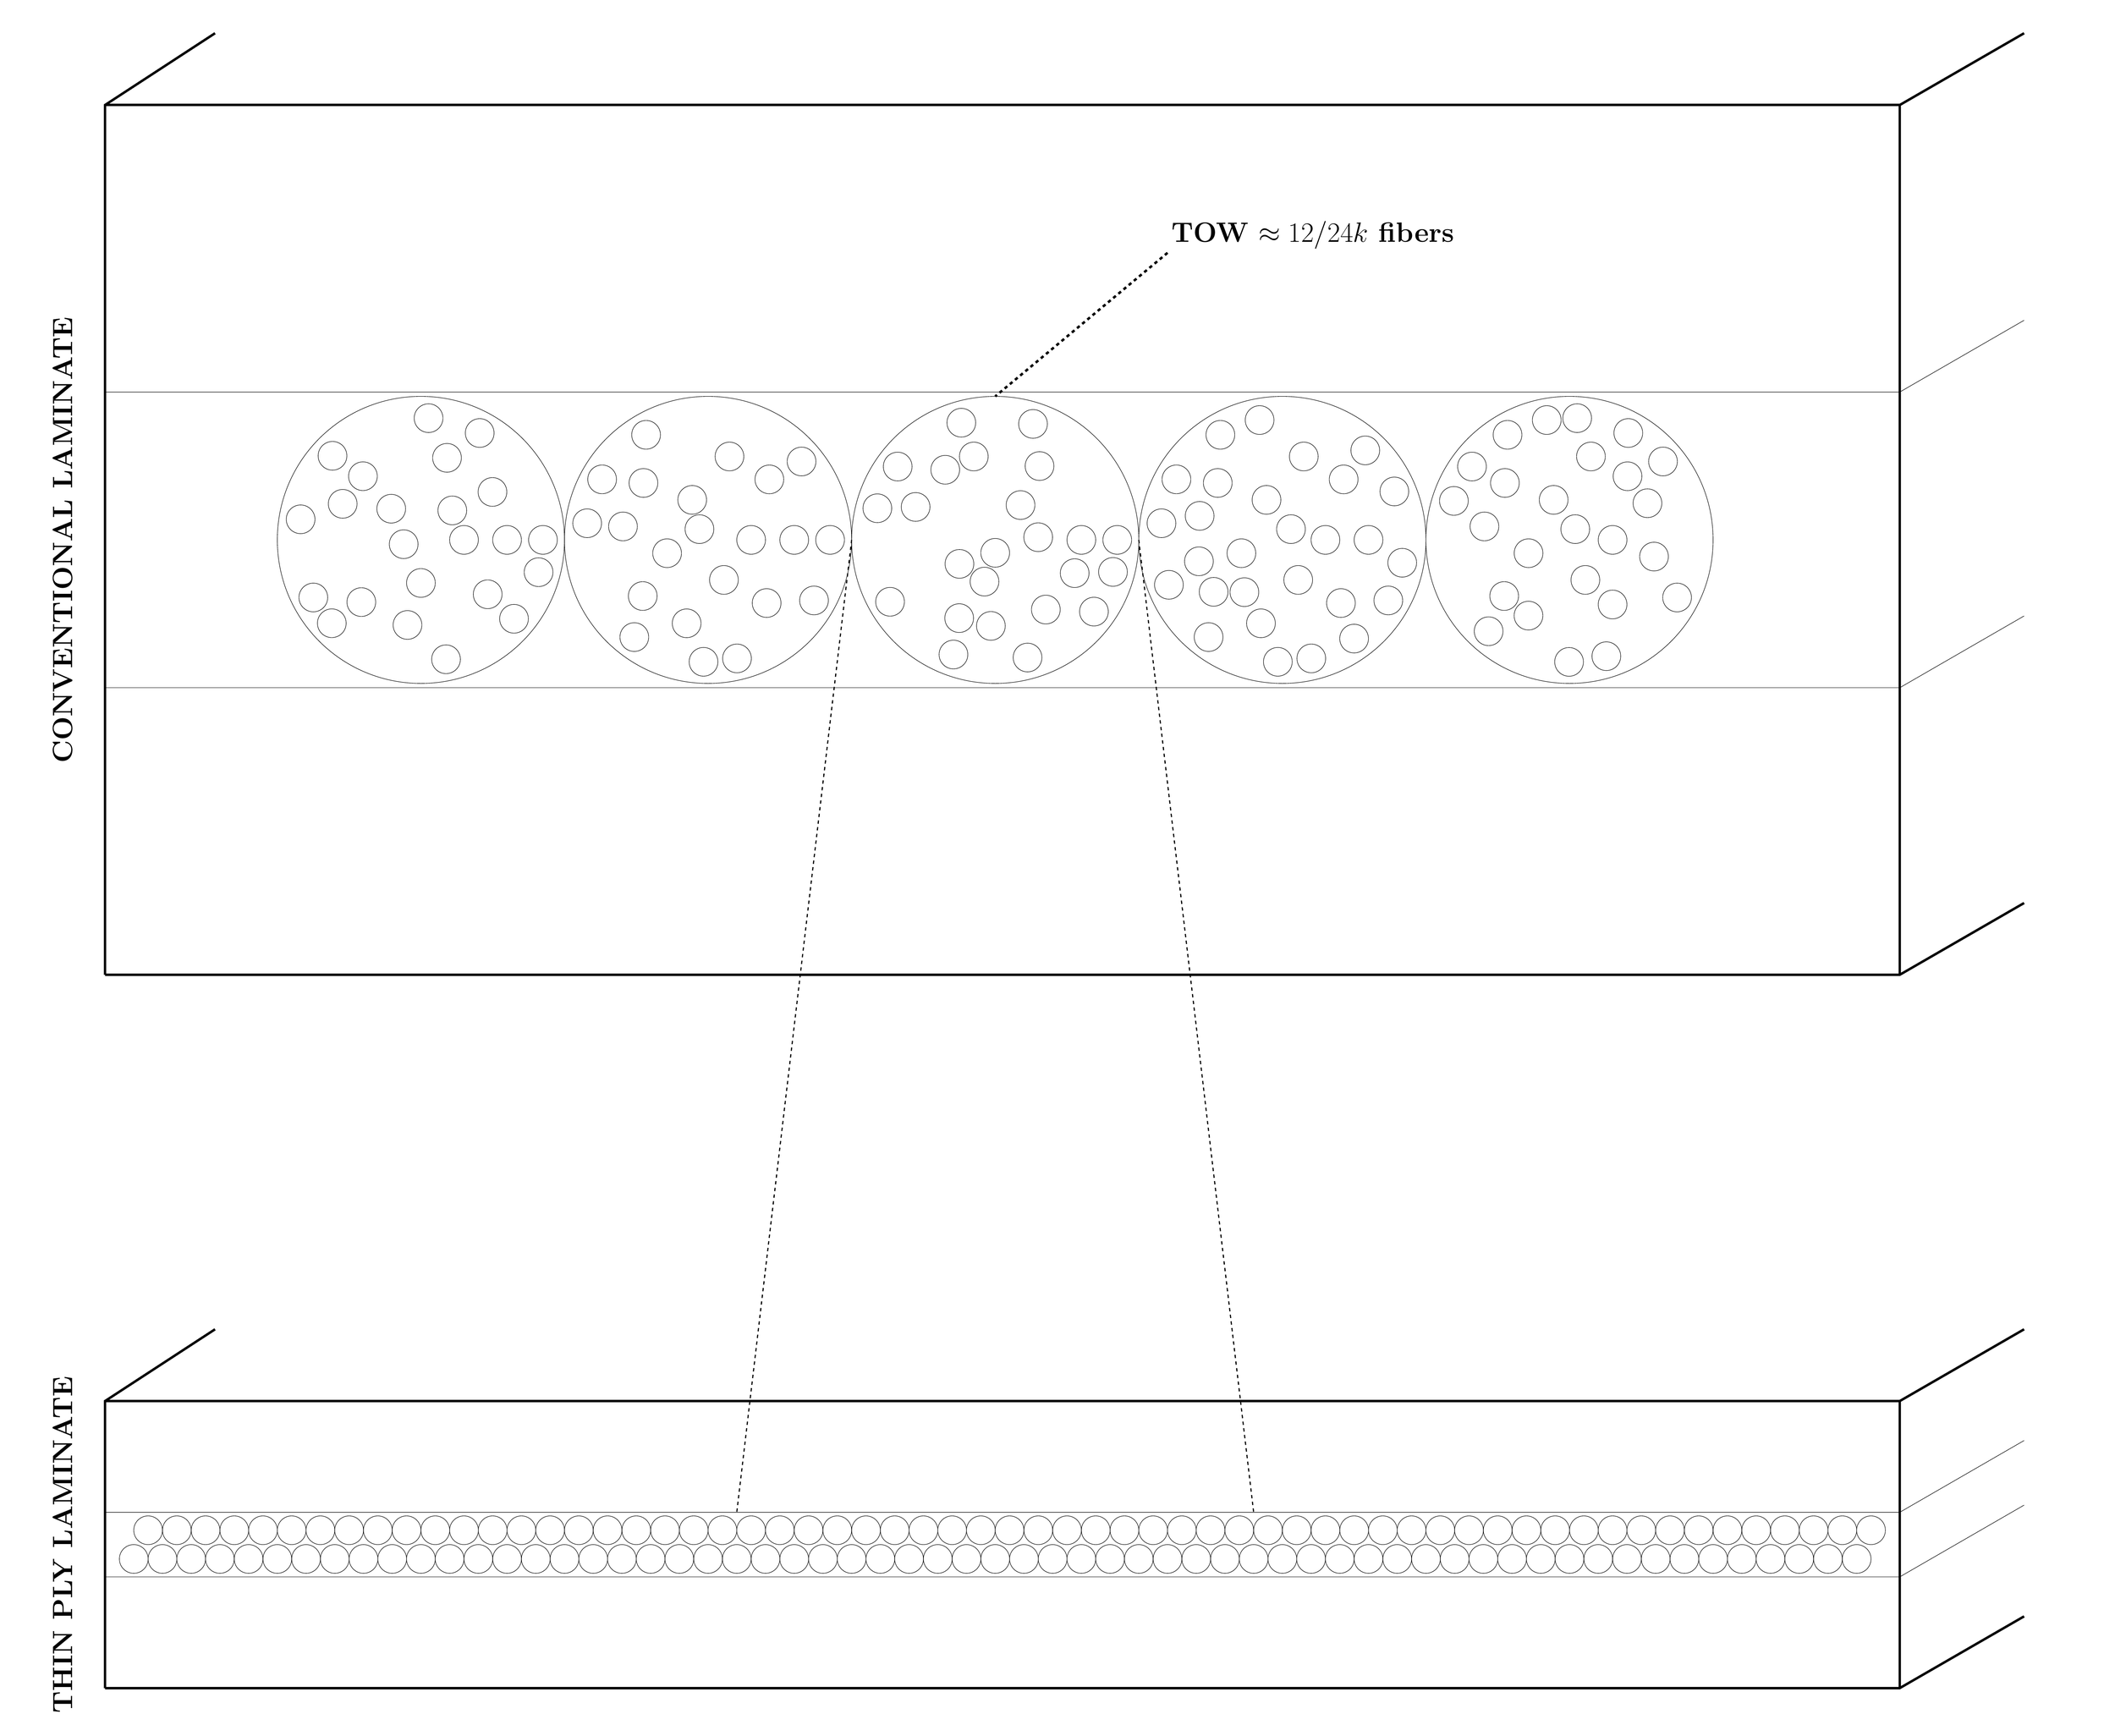
\begin{tikzpicture}[scale=4.5]
%[scale=4.5,cap=round,x=1cm,y=1cm]

%----------------------------------------------------------------------------------------------%
%                                          INPUT PARAMETERS
%----------------------------------------------------------------------------------------------%

\def\Rf{0.1}
\def\l{10}

%----------------------------------------------------------------------------------------------%
%                                        COMMAND DEFINITION
%----------------------------------------------------------------------------------------------%

\newcommand{\refSystem}[5]{
	
	\def\xlow{#1}
	\def\xup{#2}
	\def\ylow{#3}
	\def\yup{#4}

	\tikzstyle{axes}=[]

	\begin{scope}[style=axes]
 		\draw[->,draw=#5] (-\xlow,0) -- (\xup,0) ;
 		\draw[->,draw=#5] (0,-\yup) -- (0,\yup) ;
	\end{scope}
}

\newcommand{\drawFiber}[6]{
	%#1 -> Rf
	%#2 -> theta
	%#3 -> deltatheta
	%#4 -> line color
	%#5 -> x0
	%#6 -> y0

	\def\R{#1}
	\def\thetavalue{#2}
	\def\dtheta{#3}
	\def\x{#5}
	\def\y{#6}
	
	\pgfmathsetmacro\costhetaup{cos(\thetavalue+\dtheta)}
	\pgfmathsetmacro\sinthetaup{sin(\thetavalue+\dtheta)}
	
	\pgfmathsetmacro\costhetabot{cos(\thetavalue-\dtheta)}
	\pgfmathsetmacro\sinthetabot{sin(\thetavalue-\dtheta)}
	
	\def\thetaround{360+\thetavalue-\dtheta}
	
	%draw fiber surface
	\draw[draw=#4] (\x+\R*\costhetaup,\y+\R*\sinthetaup)arc (\thetavalue+\dtheta:\thetaround:\R);
	%draw radius
	%\draw[dashed](0,0)--(-\costhetabot,\sinthetabot);

}

\pgfmathsetmacro\cosproj{cos(30)}
\pgfmathsetmacro\sinproj{sin(30)}

%\refSystem{-40*2*\Rf}{35*2*\Rf}{-15*2*\Rf}{35*2*\Rf}{white};

\pgfmathsetmacro\transl{40*\Rf}

\foreach \n in {-30,-29,-28,-27,-26,-25,-24,-23,-22,-21,-20,-19,-18,-17,-16,-15,-14,-13,-12,-11,-10,-9,-8,-7,-6,-5,-4,-3,-2,-1,0,1,2,3,4,5,6,7,8,9,10,11,12,13,14,15,16,17,18,19,20,21,22,23,24,25,26,27,28,29,30}{
	\drawFiber{\Rf}{0}{360}{black}{\n*2*\Rf}{-\Rf-\transl};
}
\foreach \n in {-30,-29,-28,-27,-26,-25,-24,-23,-22,-21,-20,-19,-18,-17,-16,-15,-14,-13,-12,-11,-10,-9,-8,-7,-6,-5,-4,-3,-2,-1,0,1,2,3,4,5,6,7,8,9,10,11,12,13,14,15,16,17,18,19,20,21,22,23,24,25,26,27,28,29,30}{
	\drawFiber{\Rf}{0}{360}{black}{\n*2*\Rf+\Rf}{\Rf-\transl};
}

\draw(-31*2*\Rf,-2.25*\Rf-\transl) -- (31.5*2*\Rf,-2.25*\Rf-\transl) --  (31.5*2*\Rf+10*\Rf*\cosproj,-2.25*\Rf-\transl+10*\Rf*\sinproj)  ;
\draw(-31*2*\Rf,2.25*\Rf-\transl) -- (31.5*2*\Rf,2.25*\Rf-\transl) --  (31.5*2*\Rf+10*\Rf*\cosproj,2.25*\Rf-\transl+10*\Rf*\sinproj)  ;
\draw[line width=0.75mm](-31*2*\Rf,-10*\Rf-\transl) -- (-31*2*\Rf,10*\Rf-\transl) --  (-31.5*2*\Rf+10*\Rf*\cosproj,10*\Rf-\transl+10*\Rf*\sinproj)  ;
\draw[line width=0.75mm](31.5*2*\Rf,-10*\Rf-\transl) -- (31.5*2*\Rf,10*\Rf-\transl) -- (31.5*2*\Rf+10*\Rf*\cosproj,10*\Rf-\transl+10*\Rf*\sinproj)  ;
\draw[line width=0.75mm](-31*2*\Rf,-10*\Rf-\transl) -- (31.5*2*\Rf,-10*\Rf-\transl) -- (31.5*2*\Rf+10*\Rf*\cosproj,-10*\Rf-\transl+10*\Rf*\sinproj)  ;
\draw[line width=0.75mm](-31*2*\Rf,10*\Rf-\transl) -- (31.5*2*\Rf,10*\Rf-\transl) ;

\node[rotate=90,anchor=south] at (-32*2*\Rf,-\transl) {\Huge \bf{THIN PLY LAMINATE}};
\node[rotate=90,anchor=south] at (-34*2*\Rf,-\transl) {};

\def\Rt{10*\Rf}

\foreach \n in {-2,-1,0,1,2}{
	\pgfmathsetmacro\xt{\n*2*\Rt}
	\pgfmathsetmacro\yt{3*\Rt}
	\drawFiber{\Rt}{0}{360}{black}{\xt}{\yt};
}

\def\n{-2}
\pgfmathsetmacro\xt{\n*2*\Rt}
\pgfmathsetmacro\yt{3*\Rt}
\drawFiber{\Rf}{0}{360}{black}{1.03*\xt}{0.99*\yt};
\foreach \m in {0.,0.12,0.371,0.75}{
	\pgfmathsetmacro\cospsi{cos(\m*360.0)}
	\pgfmathsetmacro\sinpsi{sin(\m*360.0)}
	\drawFiber{\Rf}{0}{360}{black}{\xt+0.3*\Rt*\cospsi}{\yt+0.3*\Rt*\sinpsi};
}
\foreach \m in {0,0.094,0.201,0.3675,0.4312,0.62843,0.7251,0.89119}{
	\pgfmathsetmacro\cospsi{cos(\m*360.0)}
	\pgfmathsetmacro\sinpsi{sin(\m*360.0)}
	\drawFiber{\Rf}{0}{360}{black}{\xt+0.6*\Rt*\cospsi}{\yt+0.6*\Rt*\sinpsi};
}
\foreach \m in {0,0.17,.24,0.37893,0.473,0.57823,0.6197,0.783,0.8881,0.95735}{
	\pgfmathsetmacro\cospsi{cos(\m*360.0)}
	\pgfmathsetmacro\sinpsi{sin(\m*360.0)}
	\drawFiber{\Rf}{0}{360}{black}{\xt+0.85*\Rt*\cospsi}{\yt+0.85*\Rt*\sinpsi};
}

\def\n{-1}
\pgfmathsetmacro\xt{\n*2*\Rt}
\pgfmathsetmacro\yt{3*\Rt}
\drawFiber{\Rf}{0}{360}{black}{1.03*\xt}{1.025*\yt};
\foreach \m in {-0.19,0,0.31,0.55}{
	\pgfmathsetmacro\cospsi{cos(\m*360.0)}
	\pgfmathsetmacro\sinpsi{sin(\m*360.0)}
	\drawFiber{\Rf}{0}{360}{black}{\xt+0.3*\Rt*\cospsi}{\yt+0.3*\Rt*\sinpsi};
}
\foreach \m in {0,0.124,0.21,0.385,0.475,0.613,0.71,0.869}{
	\pgfmathsetmacro\cospsi{cos(\m*360.0)}
	\pgfmathsetmacro\sinpsi{sin(\m*360.0)}
	\drawFiber{\Rf}{0}{360}{black}{\xt+0.6*\Rt*\cospsi}{\yt+0.6*\Rt*\sinpsi};
}
\foreach \m in {0,0.1111,0.3347891,0.417345,0.47823,0.6467,0.7441,0.7881,0.91735}{
	\pgfmathsetmacro\cospsi{cos(\m*360.0)}
	\pgfmathsetmacro\sinpsi{sin(\m*360.0)}
	\drawFiber{\Rf}{0}{360}{black}{\xt+0.85*\Rt*\cospsi}{\yt+0.85*\Rt*\sinpsi};
}

\def\n{0}
\pgfmathsetmacro\xt{\n*2*\Rt}
\pgfmathsetmacro\yt{3*\Rt}
\drawFiber{\Rf}{0}{360}{black}{0.985*\xt}{0.97*\yt};
\foreach \m in {0.01,0.15,0.594,0.71}{
	\pgfmathsetmacro\cospsi{cos(\m*360.0)}
	\pgfmathsetmacro\sinpsi{sin(\m*360.0)}
	\drawFiber{\Rf}{0}{360}{black}{\xt+0.3*\Rt*\cospsi}{\yt+0.3*\Rt*\sinpsi};
}
\foreach \m in {0,0.164,0.29,0.3485,0.4375,0.6813,0.742,0.85,0.9369}{
	\pgfmathsetmacro\cospsi{cos(\m*360.0)}
	\pgfmathsetmacro\sinpsi{sin(\m*360.0)}
	\drawFiber{\Rf}{0}{360}{black}{\xt+0.6*\Rt*\cospsi}{\yt+0.6*\Rt*\sinpsi};
}
\foreach \m in {0,0.9,.199854,0.2947891,0.397345,0.45823,0.58467,0.69441,0.7927,0.957735}{
	\pgfmathsetmacro\cospsi{cos(\m*360.0)}
	\pgfmathsetmacro\sinpsi{sin(\m*360.0)}
	\drawFiber{\Rf}{0}{360}{black}{\xt+0.85*\Rt*\cospsi}{\yt+0.85*\Rt*\sinpsi};
}

\draw[line width=0.35mm,dashed](\xt+\Rt,\yt) -- (\xt+\Rt+8*\Rf,2.25*\Rf-\transl);
\draw[line width=0.35mm,dashed](\xt-\Rt,\yt) -- (\xt-\Rt-8*\Rf,2.25*\Rf-\transl);

\def\n{1}
\pgfmathsetmacro\xt{\n*2*\Rt}
\pgfmathsetmacro\yt{3*\Rt}
\drawFiber{\Rf}{0}{360}{black}{1.03*\xt}{1.025*\yt};
\foreach \m in {-0.19,0,0.31,0.55}{
	\pgfmathsetmacro\cospsi{cos(\m*360.0)}
	\pgfmathsetmacro\sinpsi{sin(\m*360.0)}
	\drawFiber{\Rf}{0}{360}{black}{\xt+0.3*\Rt*\cospsi}{\yt+0.3*\Rt*\sinpsi};
}
\foreach \m in {0,0.124,0.21,0.385,0.455,0.54,0.603,0.71,0.869}{
	\pgfmathsetmacro\cospsi{cos(\m*360.0)}
	\pgfmathsetmacro\sinpsi{sin(\m*360.0)}
	\drawFiber{\Rf}{0}{360}{black}{\xt+0.6*\Rt*\cospsi}{\yt+0.6*\Rt*\sinpsi};
}
\pgfmathsetmacro\cospsi{cos(0.65*360.0)}
\pgfmathsetmacro\sinpsi{sin(0.65*360.0)}
\drawFiber{\Rf}{0}{360}{black}{\xt+0.45*\Rt*\cospsi}{\yt+0.45*\Rt*\sinpsi};
\foreach \m in {0.065,0.13111,.279854,0.3347891,0.417345,0.47823,0.56,0.6467,0.7441,0.7881,0.85,0.91735,0.97}{
	\pgfmathsetmacro\cospsi{cos(\m*360.0)}
	\pgfmathsetmacro\sinpsi{sin(\m*360.0)}
	\drawFiber{\Rf}{0}{360}{black}{\xt+0.85*\Rt*\cospsi}{\yt+0.85*\Rt*\sinpsi};
}

\def\n{2}
\pgfmathsetmacro\xt{\n*2*\Rt}
\pgfmathsetmacro\yt{3*\Rt}
\drawFiber{\Rf}{0}{360}{black}{1.01*\xt}{1.025*\yt};
\drawFiber{\Rf}{0}{360}{black}{1.075*\xt}{0.85*\yt};
\foreach \m in {-0.19,0,0.31,0.55}{
	\pgfmathsetmacro\cospsi{cos(\m*360.0)}
	\pgfmathsetmacro\sinpsi{sin(\m*360.0)}
	\drawFiber{\Rf}{0}{360}{black}{\xt+0.3*\Rt*\cospsi}{\yt+0.3*\Rt*\sinpsi};
}
\foreach \m in {0.07,0.1324,0.21,0.385,0.475,0.613,0.671,0.969}{
	\pgfmathsetmacro\cospsi{cos(\m*360.0)}
	\pgfmathsetmacro\sinpsi{sin(\m*360.0)}
	\drawFiber{\Rf}{0}{360}{black}{\xt+0.6*\Rt*\cospsi}{\yt+0.6*\Rt*\sinpsi};
}
\foreach \m in {0.1111,0.17,0.24,0.279854,0.3347891,0.397345,0.44823,0.63467,0.74941,0.79881,0.921735}{
	\pgfmathsetmacro\cospsi{cos(\m*360.0)}
	\pgfmathsetmacro\sinpsi{sin(\m*360.0)}
	\drawFiber{\Rf}{0}{360}{black}{\xt+0.85*\Rt*\cospsi}{\yt+0.85*\Rt*\sinpsi};
}

\pgfmathsetmacro\ylow{0.99*3*\Rt-\Rt}
\pgfmathsetmacro\yup{1.01*3*\Rt+\Rt}
\pgfmathsetmacro\lamthick{20*\Rf}
\draw(-31*2*\Rf,\ylow) -- (31.5*2*\Rf,\ylow) --  (31.5*2*\Rf+10*\Rf*\cosproj,\ylow+10*\Rf*\sinproj)  ;
\draw(-31*2*\Rf,\yup) -- (31.5*2*\Rf,\yup) --  (31.5*2*\Rf+10*\Rf*\cosproj,\yup+10*\Rf*\sinproj)  ;
\draw[line width=0.75mm](-31*2*\Rf,\ylow-\lamthick) -- (-31*2*\Rf,\yup+\lamthick) --  (-31.5*2*\Rf+10*\Rf*\cosproj,\yup+\lamthick+10*\Rf*\sinproj)  ;
\draw[line width=0.75mm](31.5*2*\Rf,\ylow-\lamthick) -- (31.5*2*\Rf,\yup+\lamthick) -- (31.5*2*\Rf+10*\Rf*\cosproj,\yup+\lamthick+10*\Rf*\sinproj)  ;
\draw[line width=0.75mm](-31*2*\Rf,\ylow-\lamthick) -- (31.5*2*\Rf,\ylow-\lamthick) -- (31.5*2*\Rf+10*\Rf*\cosproj,\ylow-\lamthick+10*\Rf*\sinproj)  ;
\draw[line width=0.75mm](-31*2*\Rf,\yup+\lamthick) -- (31.5*2*\Rf,\yup+\lamthick) ;

\draw[line width=0.75mm,dashed](12*\Rf,5*\Rt) -- (0,4*\Rt);
\node[anchor=south west] at (12*\Rf,5*\Rt) {\Huge \bf{TOW $\approx12/24k$ fibers}};

\node[rotate=90,anchor=south] at (-32*2*\Rf,3*\Rt) {\Huge \bf{CONVENTIONAL LAMINATE}};
\node[rotate=90,anchor=north] at (34*2*\Rf+10*\Rf*\cosproj,-\transl) {};
\node[anchor=north] at (0,-12*\Rf-\transl) {};
\node[anchor=south] at (0,\yup+\lamthick+12*\Rf*\sinproj) {};


\end{tikzpicture}

\end{document}